\section{Results}
\label{s:results}

In order to extract the \ttZ and \ttW cross sections, nine signal regions (\SSLSR, 
\TLSRA, \TLSRB, \TLSRC, \TLSRD, \FLSRB, \FLSRC, \FLSRD, \FLSRE) and two control regions
(\TLCR, \FLCR) are simultaneously fitted. 
The \SSLSR\ signal region is particularly sensitive to \ttW, the \TLSRD\ signal region 
is sensitive to both, \ttW and \ttZ, while all other signal regions aim at the determination
of the \ttZ cross section.
The cross sections \sttZ and \sttW are determined using a binned maximum-likelihood fit
to the numbers of events in these regions. 
The fit is based on the profile-likelihood
technique, where systematic uncertainties are allowed to vary as nuisance
parameters and take on their best-fit values.  None of the uncertainties are
found to be significantly constrained or pulled from their initial values.  The calculation of confidence intervals and
hypothesis testing is performed using a modified frequentist method as implemented in RooStats~\cite{RooFit,RooFitManual}.

A summary of the fit to all regions used to measure the \ttZ and \ttW
production cross sections are shown in Figure~\ref{fig:allyields}.  The
normalisation corrections for the $WZ$ and $ZZ$ backgrounds with respect to the
Standard Model predictions are obtained from the fits as described in
Section~\ref{s:selection} and found to be compatible with unity: 
$1.11 \pm 0.30$
for the $WZ$ background and
$0.94 \pm 0.17$
for the $ZZ$ background.
\vspace{1ex}

\begin{figure}[htbp]
\centering
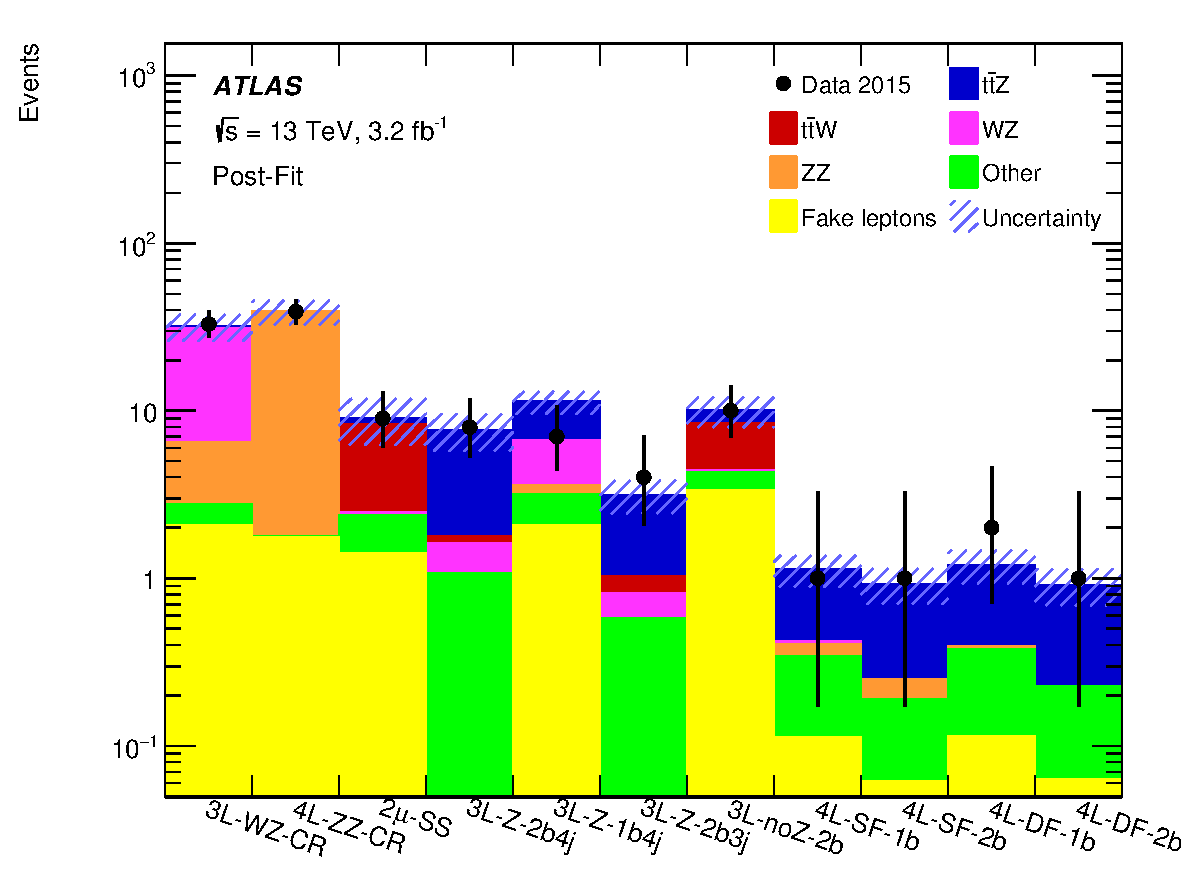
\includegraphics[width=0.85\textwidth]{Summary_ttWZ}
\caption{Expected yields after the fit compared to data for the
fit to extract \sttZ and \sttW in the signal regions and in the control regions
used to constrain the $WZ$ and $ZZ$ backgrounds.  The `Other' background
summarises all other backgrounds described in Section~\ref{s:samples}.  
\hatch.\label{fig:allyields}}
\end{figure}

The results of the fit are $\sigma_{\ttZ} = 0.92 \pm 0.29 \stat \pm 0.10 \syst$
pb and $\sigma_{\ttW} = 1.50 \pm 0.72 \stat \pm 0.33 \syst$ pb with a
correlation of $-0.13$ and are shown in Figure~\ref{fig:simfit}.  The fit
yields significances of $3.9\sigma$ and $2.2\sigma$ over the background-only
hypothesis for the \ttZ and \ttW processes, respectively. The expected
significances are $3.4\sigma$ for \ttZ and $1.0\sigma$ for \ttW production.
The significance values are computed using the asymptotic approximation described in Ref.~\cite{cls_3}. 
%
In the two channels most sensitive to the \ttW signal the observed relative
number of events with two positively or two negatively charged leptons
is compatible with expectation. In the \TLSRD\ channel the observed distribution of 
the number of events with a given amount of electrons and muons match expectation, as well.

\begin{figure}[htbp]
\centering
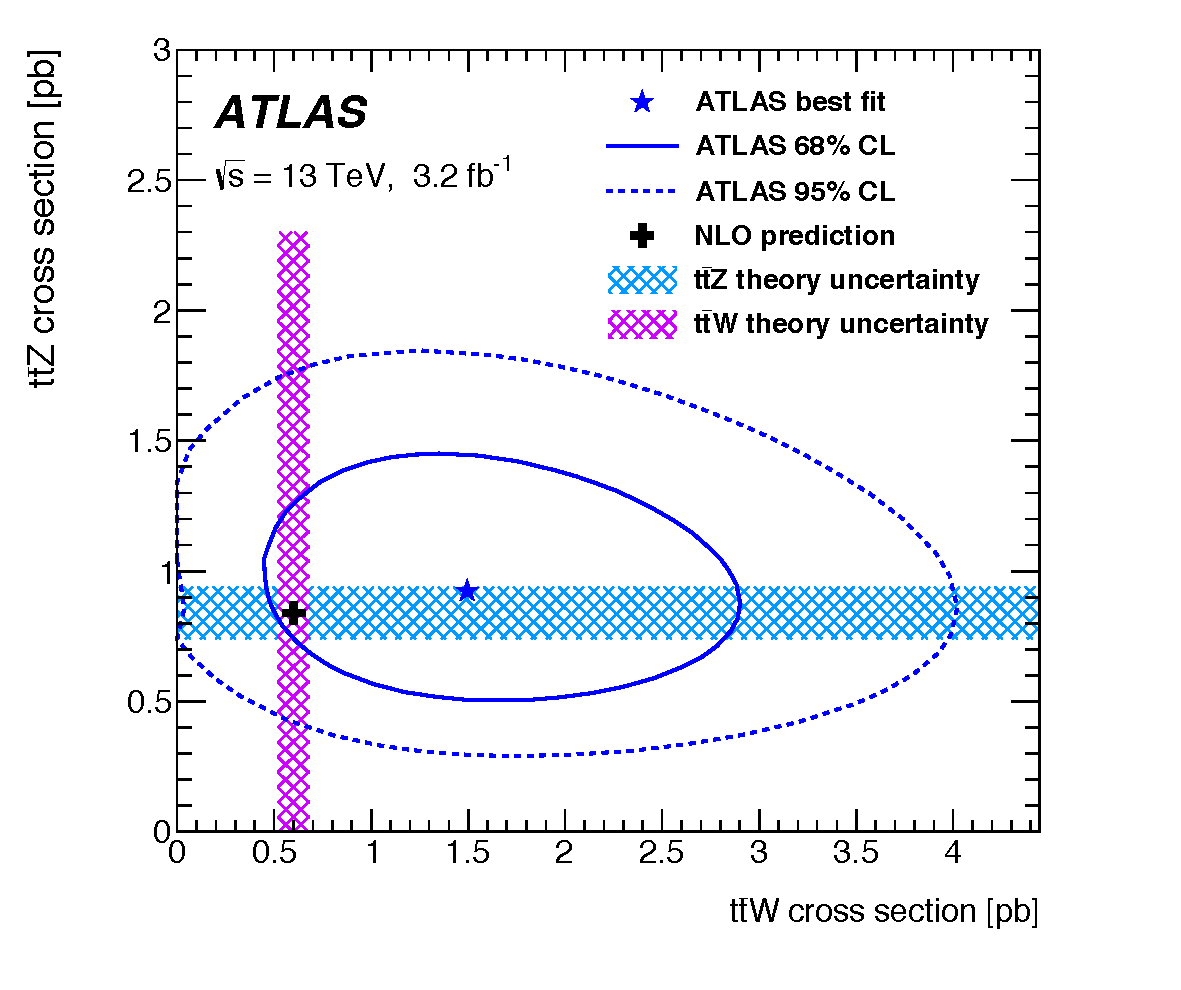
\includegraphics[width=0.85\textwidth]{ttZ_vs_ttW_2Dfit}
\caption{The result of the simultaneous fit to the \ttZ and \ttW cross sections
along with the 68\% and 95\% confidence level (CL) contours. The shaded areas
correspond to the theoretical uncertainties in the Standard Model predictions,
and include renormalisation and factorisation scale uncertainties as well as
PDF uncertainties including $\alphas$ variations.}
\label{fig:simfit}
\end{figure}

Table~\ref{tab:syst} shows the leading and total uncertainties in the
measured \ttZ and \ttW cross sections. In estimating the uncertainties for \ttZ (\ttW), the cross section for \ttW (\ttZ) is fixed to its
Standard Model value. For both processes, the precision of
the measurement is dominated by statistical uncertainties.  For the \ttZ determination,
the different sources contribute with similar size to the total systematic uncertainty.
For the \ttW determination, the dominant systematic uncertainty source is
the limited amount of data available for the estimation of the fake leptons.

\begin{table}[htbp]
\centering \renewcommand{\arraystretch}{1.2}
\caption{List of dominant and total uncertainties in the measured cross 
sections of the \ttZ and \ttW processes from the fit. All uncertainties are
symmetrised.\vspace{1ex}}
\label{tab:syst}
\begin{tabular}{lcc}
\toprule
Uncertainty                 &   $\sigma_{\ttZ}$ & $\sigma_{\ttW}$ \\
\midrule
Luminosity                    & 2.6\% & 3.1\%  \\
Reconstructed objects         & 8.3\% & 9.3\%  \\
Backgrounds from simulation   & 5.3\% & 3.1\%  \\
Fake leptons and charge misID & 3.0\% & 19\%  \\
Signal modelling   & 2.3\% & 4.2\%  \\
\midrule
Total systematic            & 11\% & 22\% \\
Statistical                 & 31\% & 48\% \\
\midrule
Total                       & 32\% & 53\% \\
\bottomrule
\end{tabular}
\end{table}
